\documentclass[a4paper,12pt]{article}
\usepackage[ukrainian,english]{babel}
\usepackage{ucs}
\usepackage[utf8]{inputenc}
\usepackage[T2A]{fontenc}
\usepackage{amsmath}
\usepackage{amsfonts}
\usepackage{graphicx}
\usepackage{pdflscape}
\usepackage{lscape,lipsum,graphicx}
\usepackage[absolute]{textpos}
\usepackage{fancyhdr}
\usepackage[paper=portrait,pagesize]{typearea}
\makeatletter
\newcommand{\skipitems}[1]{%
  \addtocounter{\@enumctr}{#1}%
}
\makeatother
\usepackage[table,xcdraw]{xcolor}
\newcommand\tab[1][1cm]{\hspace*{#1}}
\usepackage[left=20mm, top=20mm, right=10mm, bottom=20mm, nohead, nofoot]{geometry}
\begin{document}
\begin{center}
{\LARGE Домашня робота 3}	
\end{center}
\begin{enumerate}
	\item \begin{enumerate} 
	\item $(\neg(Q\rightarrow(\neg ((\neg P)\leftrightarrow(\neg R))))\rightarrow(((\neg P)\lor Q)\lor R));\\(\neg(\mathbb{F}\rightarrow(\neg ((\neg \mathbb{T})\leftrightarrow(\neg \mathbb{T}))))\rightarrow(((\neg \mathbb{T})\lor \mathbb{F})\lor \mathbb{T}));\\(\neg(\mathbb{F}\rightarrow(\neg \mathbb{T}))\rightarrow( \mathbb{F}\lor \mathbb{T}));\tab \underbrace{((\neg \mathbb{T})\rightarrow\mathbb{F})}_{\mathbb{T}}$
	\item $((P\lor(\neg((\neg S)\rightarrow(\neg R))))\leftrightarrow((\neg P)\rightarrow Q));\\((\mathbb{T}\lor(\neg((\neg \mathbb{F})\rightarrow(\neg \mathbb{T}))))\leftrightarrow((\neg \mathbb{T})\rightarrow \mathbb{F}));\\((\mathbb{T}\lor(\neg \mathbb{F}))\leftrightarrow \mathbb{T});\tab \underbrace{(\mathbb{T}\leftrightarrow\mathbb{T})}_{\mathbb{T}}$
	\end{enumerate}
	\item \begin{enumerate} \item $A=P\land Q;\>\>B=(P\lor Q)	\rightarrow(\neg P\rightarrow\neg Q)$
\begin{table}[!htb]

    \begin{minipage}{.4\linewidth}
      \centering
        \begin{tabular}{|c|c|c|}
\hline
$P$            & $Q$            & $P\land Q$                           \\ \hline
$\mathbb{T}$ & $\mathbb{T}$ & $\mathbb{T}$                         \\ 
$\mathbb{T}$ & $\mathbb{F}$ & \cellcolor[HTML]{FFCCC9}$\mathbb{F}$ \\
$\mathbb{F}$ & $\mathbb{T}$ & \cellcolor[HTML]{FFCCC9}$\mathbb{F}$ \\
$\mathbb{F}$ & $\mathbb{F}$ & \cellcolor[HTML]{FFCCC9}$\mathbb{F}$ \\ \hline
\end{tabular}
    \end{minipage}%
    \begin{minipage}{.3\linewidth}
      \centering
        \begin{tabular}{|c|c|c|c|c|c|c|}
\hline
$P$            & $Q$            & $\neg P$     & $\neg Q$     & $P\lor Q$    & $\neg P\lor \neg Q$ & $B$          \\ \hline
$\mathbb{T}$ & $\mathbb{T}$ & $\mathbb{F}$ & $\mathbb{F}$ & $\mathbb{T}$ & $\mathbb{T}$        & $\mathbb{T}$ \\ 
\rowcolor[HTML]{FFCCC9} 
             &              &              &              &              &                     &              \\ 
\rowcolor[HTML]{FFCCC9} 
             &              &              &              &              &                     &              \\ 
\rowcolor[HTML]{FFCCC9} 
             &              &              &              &              &                     &              \\ \hline
\end{tabular} 
    \end{minipage} 
\end{table}\\
$\Rightarrow $ Якщо $A$ приймає значення $\mathbb{T}$, то і $B$ приймає значення $\mathbb{T}$.
\item $A=P\lor Q;\>\>B=P\leftrightarrow Q$
\begin{table}[!htb]
    \begin{minipage}{.4\linewidth}
      \centering
        \begin{tabular}{|c|c|c|}
\hline
$P$          & $Q$          & $P\lor Q$                            \\ \hline
$\mathbb{T}$ & $\mathbb{T}$ & $\mathbb{T}$                         \\ 
$\mathbb{T}$ & $\mathbb{F}$ & $\mathbb{T}$                         \\ 
$\mathbb{F}$ & $\mathbb{T}$ & $\mathbb{T}$                         \\ 
$\mathbb{F}$ & $\mathbb{F}$ & \cellcolor[HTML]{FFCCC9}$\mathbb{F}$ \\ \hline
\end{tabular}
    \end{minipage}%
    \begin{minipage}{.4\linewidth}
      \centering

        \begin{tabular}{|c|c|c|}
\hline
$P$          & $Q$          & $P\leftrightarrow Q$ \\ \hline
$\mathbb{T}$ & $\mathbb{T}$ & $\mathbb{T}$         \\ 
$\mathbb{T}$ & $\mathbb{F}$ & $\mathbb{F}$         \\ 
$\mathbb{F}$ & $\mathbb{T}$ & $\mathbb{F}$         \\ 
\rowcolor[HTML]{FFCCC9} 
 &  &         \\ \hline
\end{tabular}
    \end{minipage} 
\end{table}\\
$\Rightarrow$  нічого не можно сказати.
\end{enumerate}
\item $(((P\rightarrow Q)\lor R)\rightarrow\underbrace{((P\rightarrow(\neg Q))\rightarrow (\neg(P\rightarrow(\neg R))))}_{=B})=A$
\begin{table}[htp]
\centering
\begin{tabular}{|c|c|c|c|c|c|c|c|c|c|c|c|}
\hline
\multicolumn{1}{|c|}{$P$} & \multicolumn{1}{c|}{$Q$} & \multicolumn{1}{c|}{$R$} & \multicolumn{1}{c|}{$\neg Q$} & \multicolumn{1}{c|}{$\neg R$} & \multicolumn{1}{c|}{$P\rightarrow Q$} & \multicolumn{1}{c|}{$P\rightarrow Q\lor R$} & \multicolumn{1}{c|}{$P\rightarrow\neg Q$} & \multicolumn{1}{c|}{$P\rightarrow\neg R$} & \multicolumn{1}{c|}{$\neg(P\rightarrow\neg R)$} & \multicolumn{1}{c|}{$B$} & \multicolumn{1}{c|}{$A$}               \\ \hline
$\mathbb{T}$                & $\mathbb{T}$             & $\mathbb{T}$             & $\mathbb{F}$                  & $\mathbb{F}$                  & $\mathbb{T}$                          & $\mathbb{T}$                                & $\mathbb{F}$                              & $\mathbb{F}$                              & $\mathbb{T}$                                    & $\mathbb{T}$                                                                     & $\mathbb{T}$                         \\
$\mathbb{T}$                & $\mathbb{T}$             & $\mathbb{F}$             & $\mathbb{F}$                  & $\mathbb{T}$                  & $\mathbb{T}$                          & $\mathbb{T}$                                & $\mathbb{F}$                              & $\mathbb{T}$                              & $\mathbb{F}$                                    & $\mathbb{T}$                                                                     & $\mathbb{T}$                         \\
$\mathbb{T}$                & $\mathbb{F}$             & $\mathbb{T}$             & $\mathbb{T}$                  & $\mathbb{F}$                  & $\mathbb{F}$                          & $\mathbb{T}$                                & $\mathbb{T}$                              & $\mathbb{F}$                              & $\mathbb{T}$                                    & $\mathbb{T}$                                                                     & $\mathbb{T}$                         \\
$\mathbb{T}$                & $\mathbb{F}$             & $\mathbb{F}$             & $\mathbb{T}$                  & $\mathbb{T}$                  & $\mathbb{F}$                          & $\mathbb{F}$                                & $\mathbb{T}$                              & $\mathbb{T}$                              & $\mathbb{F}$                                    & $\mathbb{F}$                                                                     & $\mathbb{T}$                         \\
$\mathbb{F}$                & $\mathbb{T}$             & $\mathbb{T}$             & $\mathbb{F}$                  & $\mathbb{F}$                  & $\mathbb{T}$                          & $\mathbb{T}$                                & $\mathbb{T}$                              & $\mathbb{T}$                              & $\mathbb{F}$                                    & $\mathbb{F}$                                                                     & \cellcolor[HTML]{FFCCC9}$\mathbb{F}$ \\
$\mathbb{F}$                & $\mathbb{T}$             & $\mathbb{F}$             & $\mathbb{F}$                  & $\mathbb{T}$                  & $\mathbb{T}$                          & $\mathbb{T}$                                & $\mathbb{T}$                              & $\mathbb{T}$                              & $\mathbb{F}$                                    & $\mathbb{F}$                                                                     & \cellcolor[HTML]{FFCCC9}$\mathbb{F}$ \\
$\mathbb{F}$                & $\mathbb{F}$             & $\mathbb{T}$             & $\mathbb{T}$                  & $\mathbb{F}$                  & $\mathbb{T}$                          & $\mathbb{T}$                                & $\mathbb{T}$                              & $\mathbb{T}$                              & $\mathbb{F}$                                    & $\mathbb{F}$                                                                     & \cellcolor[HTML]{FFCCC9}$\mathbb{F}$ \\
$\mathbb{F}$                & $\mathbb{F}$             & $\mathbb{F}$             & $\mathbb{T}$                  & $\mathbb{T}$                  & $\mathbb{T}$                          & $\mathbb{T}$                                & $\mathbb{T}$                              & $\mathbb{T}$                              & $\mathbb{F}$                                    & $\mathbb{F}$                                                                     & \cellcolor[HTML]{FFCCC9}$\mathbb{F}$ \\\hline
\end{tabular}
\end{table}
\\ Моделі:\tab $\{P,\>Q,\>R\},\>\>\{P,\>\neg Q,\>R\},\>\>\{P,\>Q,\>\neg R\},\>\>\{P,\>\neg Q,\>\neg R\}$
\begin{center}
	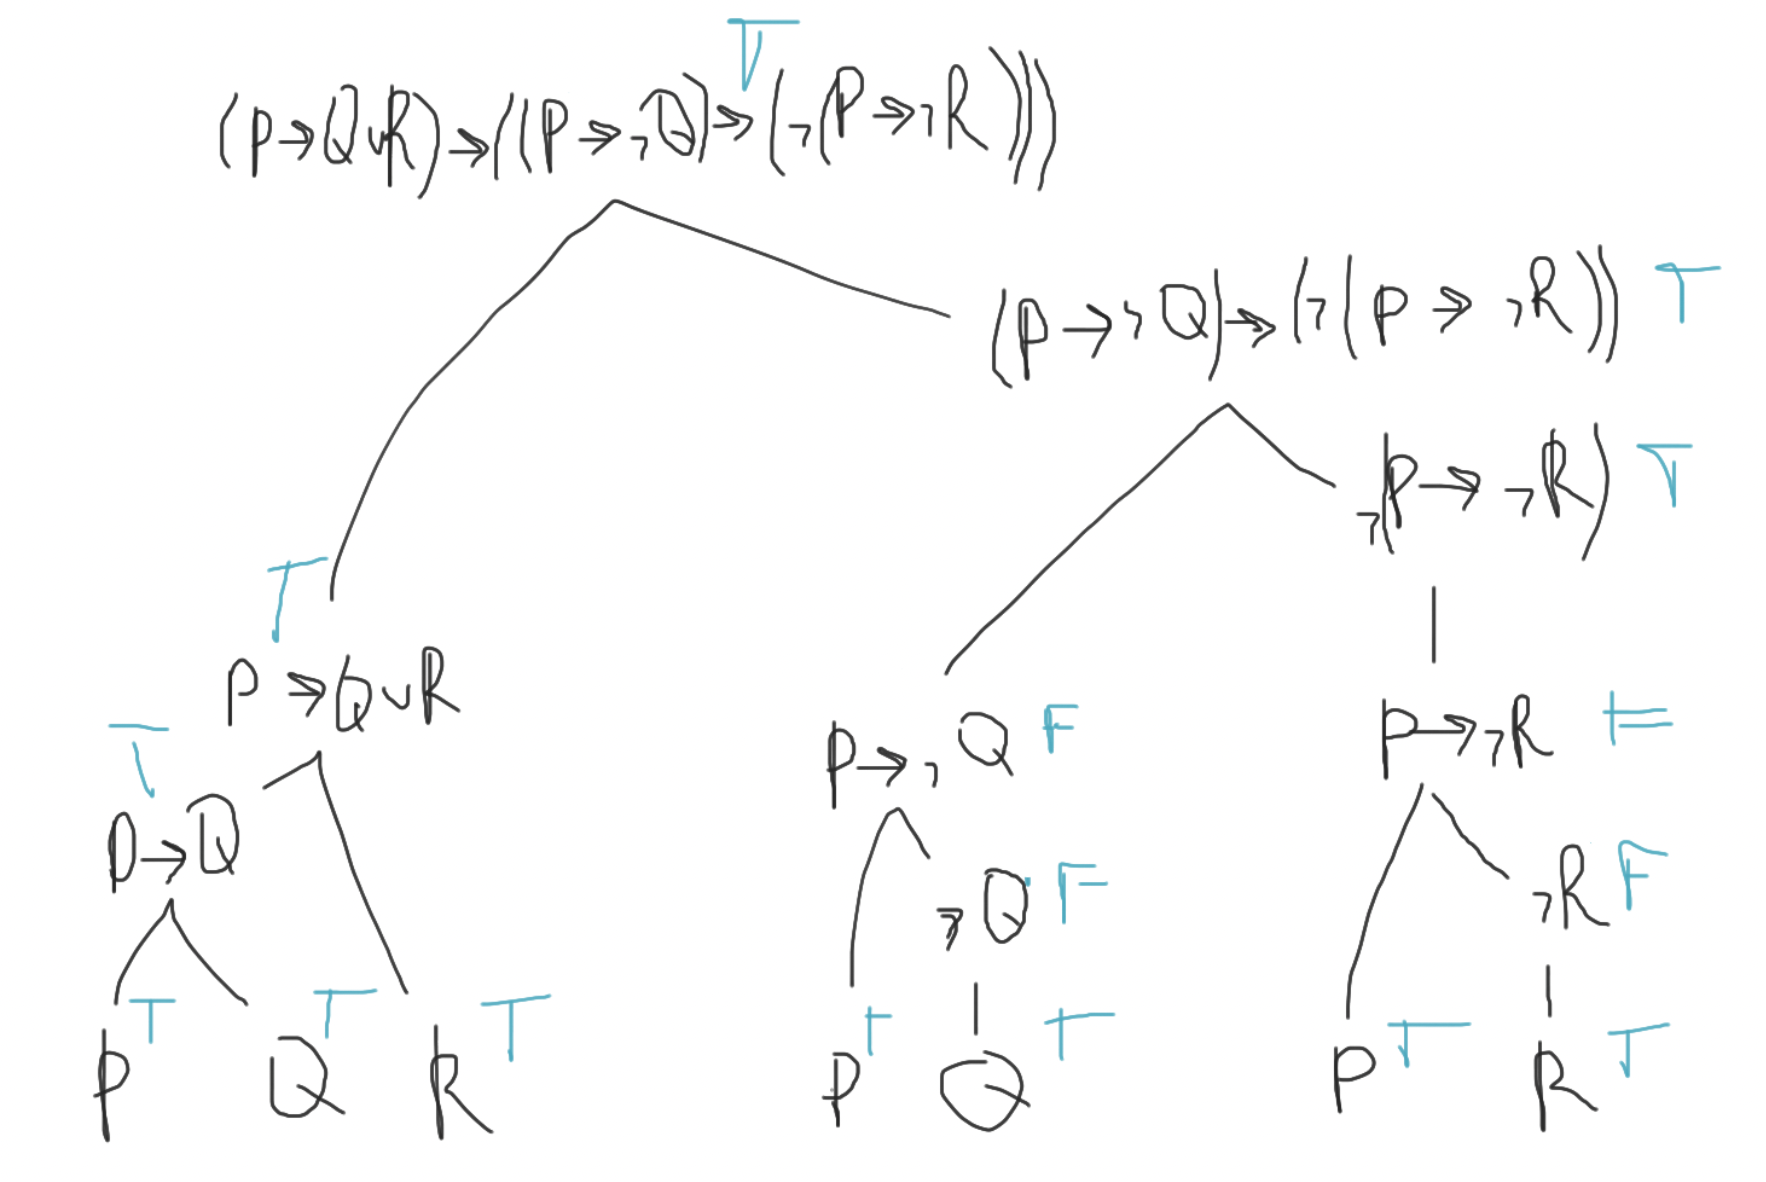
\includegraphics[height=10cm]{tree4}
\end{center}
\skipitems{1} 
\item \begin{enumerate}
\item $(A\rightarrow(P\lor Q))\rightarrow((A\rightarrow P)\rightarrow Q)$

\begin{table}[htp]
\centering
\begin{tabular}{|c|c|c|c|c|c|c|c|}
\hline
\multicolumn{1}{|c|}{$P$} & \multicolumn{1}{c|}{$Q$} & \multicolumn{1}{c|}{$A$} & \multicolumn{1}{c|}{$P\lor Q$} & \multicolumn{1}{c|}{$A\rightarrow(P\lor Q)$} & \multicolumn{1}{c|}{$(A\rightarrow P$} & \multicolumn{1}{c|}{$(A\rightarrow P)\rightarrow Q$} & \multicolumn{1}{c|}{$(A\rightarrow(P\lor Q))\rightarrow((A\rightarrow P)\rightarrow Q)$} \\ \hline
$\mathbb{T}$              & $\mathbb{T}$             & $\mathbb{T}$             & $\mathbb{F}$                   & $\mathbb{T}$                                 & $\mathbb{T}$                           & $\mathbb{F}$                                         & \cellcolor[HTML]{FFCCC9}$\mathbb{F}$                                                     \\
$\mathbb{T}$              & $\mathbb{T}$             & $\mathbb{F}$             & $\mathbb{F}$                   & $\mathbb{F}$                                 & $\mathbb{F}$                           & $\mathbb{T}$                                         & $\mathbb{T}$                                                                             \\
$\mathbb{T}$              & $\mathbb{F}$             & $\mathbb{T}$             & $\mathbb{T}$                   & $\mathbb{T}$                                 & $\mathbb{T}$                           & $\mathbb{T}$                                         & $\mathbb{T}$                                                                             \\
$\mathbb{T}$              & $\mathbb{F}$             & $\mathbb{F}$             & $\mathbb{T}$                   & $\mathbb{T}$                                 & $\mathbb{T}$                           & $\mathbb{T}$                                         & $\mathbb{T}$                                                                             \\
$\mathbb{F}$              & $\mathbb{T}$             & $\mathbb{T}$             & $\mathbb{T}$                   & $\mathbb{T}$                                 & $\mathbb{T}$                           & $\mathbb{F}$                                         & \cellcolor[HTML]{FFCCC9}$\mathbb{F}$                                                     \\
$\mathbb{F}$              & $\mathbb{T}$             & $\mathbb{F}$             & $\mathbb{T}$                   & $\mathbb{T}$                                 & $\mathbb{F}$                           & $\mathbb{T}$                                         & $\mathbb{T}$                                                                             \\
$\mathbb{F}$              & $\mathbb{F}$             & $\mathbb{T}$             & $\mathbb{T}$                   & $\mathbb{T}$                                 & $\mathbb{T}$                           & $\mathbb{T}$                                         & $\mathbb{T}$                                                                             \\
$\mathbb{F}$              & $\mathbb{F}$             & $\mathbb{F}$             & $\mathbb{T}$                   & $\mathbb{T}$                                 & $\mathbb{T}$                           & $\mathbb{T}$                                         & $\mathbb{T}$   \\\hline                                                                         
\end{tabular}
\end{table}\begin{center}
\begin{table}[!htb]
\centering
    \begin{minipage}{.2\linewidth}
      \centering
        \begin{tabular}{|c|c|c|}\hline 
$P$          & $Q$          & $A_1$        \\\hline
$\mathbb{T}$ & $\mathbb{T}$ & $\mathbb{T}$ \\
$\mathbb{T}$ & $\mathbb{F}$ & $\mathbb{F}$ \\
$\mathbb{F}$ & $\mathbb{T}$ & $\mathbb{T}$ \\
$\mathbb{F}$ & $\mathbb{F}$ & $\mathbb{T}$ \\\hline
\end{tabular}
    \end{minipage}%
    \begin{minipage}{.2\linewidth}
      \centering
        \begin{tabular}{|c|c|c|}\hline
$P$          & $Q$          & $A_2$        \\\hline
$\mathbb{T}$ & $\mathbb{T}$ & $\mathbb{F}$ \\
$\mathbb{T}$ & $\mathbb{F}$ & $\mathbb{F}$ \\
$\mathbb{F}$ & $\mathbb{T}$ & $\mathbb{T}$ \\
$\mathbb{F}$ & $\mathbb{F}$ & $\mathbb{T}$ \\\hline
\end{tabular}
    \end{minipage}%
    \begin{minipage}{.2\linewidth}
      \centering
        \begin{tabular}{|c|c|c|}\hline
$P$          & $Q$          & $A_3$        \\\hline
$\mathbb{T}$ & $\mathbb{T}$ & $\mathbb{T}$ \\
$\mathbb{T}$ & $\mathbb{F}$ & $\mathbb{F}$ \\
$\mathbb{F}$ & $\mathbb{T}$ & $\mathbb{F}$ \\
$\mathbb{F}$ & $\mathbb{F}$ & $\mathbb{T}$ \\\hline
\end{tabular}
    \end{minipage}%
    \begin{minipage}{.2\linewidth}
      \centering
        \begin{tabular}{|c|c|c|}\hline
$P$          & $Q$          & $A_4$        \\\hline
$\mathbb{T}$ & $\mathbb{T}$ & $\mathbb{F}$ \\
$\mathbb{T}$ & $\mathbb{F}$ & $\mathbb{F}$ \\
$\mathbb{F}$ & $\mathbb{T}$ & $\mathbb{F}$ \\
$\mathbb{F}$ & $\mathbb{F}$ & $\mathbb{T}$ \\\hline
\end{tabular}
    \end{minipage} 
\end{table}
\end{center}\newpage 
\item $(((\neg P)\lor(\neg Q)\land A)\rightarrow(A\rightarrow(P\land Q)) = F$
\begin{table}[htp]\centering
\begin{tabular}{|c|c|c|c|c|c|c|c|c|c|}\hline
$P$          & $Q$          & $A$          & $\neg P$     & $\neg Q$     & $\neg P\lor\neg Q$ & $(\neg P\lor\neg Q)\land A$ & $P\land Q$   & $A\rightarrow(P\land Q)$ & $F$ \\\hline
$\mathbb{T}$ & $\mathbb{T}$ & $\mathbb{T}$ & $\mathbb{F}$ & $\mathbb{F}$ & $\mathbb{T}$       & $\mathbb{F}$                & $\mathbb{F}$ & $\mathbb{T}$             & $\mathbb{T}$                                                                                                                                                           \\
$\mathbb{T}$ & $\mathbb{T}$ & $\mathbb{F}$ & $\mathbb{F}$ & $\mathbb{F}$ & $\mathbb{T}$       & $\mathbb{T}$                & $\mathbb{F}$ & $\mathbb{F}$             & \cellcolor[HTML]{FFCCC9}$\mathbb{F}$                                                                                                                                   \\
$\mathbb{T}$ & $\mathbb{F}$ & $\mathbb{T}$ & $\mathbb{F}$ & $\mathbb{T}$ & $\mathbb{T}$       & $\mathbb{F}$                & $\mathbb{F}$ & $\mathbb{T}$             & $\mathbb{T}$                                                                                                                                                           \\
$\mathbb{T}$ & $\mathbb{F}$ & $\mathbb{F}$ & $\mathbb{F}$ & $\mathbb{T}$ & $\mathbb{T}$       & $\mathbb{T}$                & $\mathbb{F}$ & $\mathbb{F}$             & \cellcolor[HTML]{FFCCC9}$\mathbb{F}$                                                                                                                                   \\
$\mathbb{F}$ & $\mathbb{T}$ & $\mathbb{T}$ & $\mathbb{T}$ & $\mathbb{F}$ & $\mathbb{T}$       & $\mathbb{F}$                & $\mathbb{F}$ & $\mathbb{T}$             & $\mathbb{T}$                                                                                                                                                           \\
$\mathbb{F}$ & $\mathbb{T}$ & $\mathbb{F}$ & $\mathbb{T}$ & $\mathbb{F}$ & $\mathbb{T}$       & $\mathbb{T}$                & $\mathbb{F}$ & $\mathbb{T}$             & $\mathbb{T}$                                                                                                                                                           \\
$\mathbb{F}$ & $\mathbb{F}$ & $\mathbb{T}$ & $\mathbb{T}$ & $\mathbb{T}$ & $\mathbb{F}$       & $\mathbb{F}$                & $\mathbb{T}$ & $\mathbb{T}$             & $\mathbb{T}$                                                                                                                                                           \\
$\mathbb{F}$ & $\mathbb{F}$ & $\mathbb{F}$ & $\mathbb{T}$ & $\mathbb{T}$ & $\mathbb{F}$       & $\mathbb{T}$                & $\mathbb{T}$ & $\mathbb{T}$             & $\mathbb{T}$ \\\hline                                                                                                                                                         
\end{tabular}
\end{table}
\begin{table}[!htb]\centering
    \begin{minipage}{.2\linewidth}
      \centering
        \begin{tabular}{|c|c|c|}\hline
$P$          & $Q$          & $A_1$        \\\hline
$\mathbb{F}$ & $\mathbb{F}$ & $\mathbb{F}$ \\
$\mathbb{F}$ & $\mathbb{T}$ & $\mathbb{F}$ \\
$\mathbb{T}$ & $\mathbb{F}$ & $\mathbb{F}$ \\
$\mathbb{T}$ & $\mathbb{T}$ & $\mathbb{F}$ \\\hline
\end{tabular}
    \end{minipage}%
    \begin{minipage}{.2\linewidth}
      \centering
        \begin{tabular}{|c|c|c|}\hline
$P$          & $Q$          & $A_2$        \\\hline
$\mathbb{F}$ & $\mathbb{F}$ & $\mathbb{F}$ \\
$\mathbb{F}$ & $\mathbb{T}$ & $\mathbb{F}$ \\
$\mathbb{T}$ & $\mathbb{F}$ & $\mathbb{F}$ \\
$\mathbb{T}$ & $\mathbb{T}$ & $\mathbb{T}$ \\\hline
\end{tabular}    \end{minipage}%
    \begin{minipage}{.2\linewidth}
      \centering
        \begin{tabular}{|c|c|c|}\hline
$P$          & $Q$          & $A_3$        \\\hline
$\mathbb{F}$ & $\mathbb{F}$ & $\mathbb{F}$ \\
$\mathbb{F}$ & $\mathbb{T}$ & $\mathbb{F}$ \\
$\mathbb{T}$ & $\mathbb{F}$ & $\mathbb{T}$ \\
$\mathbb{T}$ & $\mathbb{T}$ & $\mathbb{F}$ \\\hline
\end{tabular}
    \end{minipage}%
    \begin{minipage}{.2\linewidth}
      \centering
        \begin{tabular}{|c|c|c|}\hline
$P$          & $Q$          & $A_1$        \\\hline
$\mathbb{F}$ & $\mathbb{F}$ & $\mathbb{F}$ \\
$\mathbb{F}$ & $\mathbb{T}$ & $\mathbb{F}$ \\
$\mathbb{T}$ & $\mathbb{F}$ & $\mathbb{T}$ \\
$\mathbb{T}$ & $\mathbb{T}$ & $\mathbb{T}$ \\\hline
\end{tabular}
    \end{minipage} 
\end{table}
\end{enumerate}
\item 
\begin{enumerate}
\item $\neg(P\lor Q)\models \neg P\lor Q$
\begin{table}[!htb]\centering
    \begin{minipage}{.4\linewidth}
      \centering
        \begin{tabular}{|c|c|c|c|c|}\hline
$P$          & $Q$          & $R$          & $P\lor Q$    & $\neg(P\lor Q)$                      \\\hline
$\mathbb{T}$ & $\mathbb{T}$ & $\mathbb{T}$ & $\mathbb{T}$ & \cellcolor[HTML]{FFCCC9}$\mathbb{F}$ \\
$\mathbb{T}$ & $\mathbb{T}$ & $\mathbb{F}$ & $\mathbb{T}$ & \cellcolor[HTML]{FFCCC9}$\mathbb{F}$ \\
$\mathbb{T}$ & $\mathbb{F}$ & $\mathbb{T}$ & $\mathbb{T}$ & \cellcolor[HTML]{FFCCC9}$\mathbb{F}$ \\
$\mathbb{T}$ & $\mathbb{F}$ & $\mathbb{F}$ & $\mathbb{T}$ & \cellcolor[HTML]{FFCCC9}$\mathbb{F}$ \\
$\mathbb{F}$ & $\mathbb{T}$ & $\mathbb{T}$ & $\mathbb{T}$ & \cellcolor[HTML]{FFCCC9}$\mathbb{F}$ \\
$\mathbb{F}$ & $\mathbb{T}$ & $\mathbb{F}$ & $\mathbb{T}$ & \cellcolor[HTML]{FFCCC9}$\mathbb{F}$ \\
$\mathbb{F}$ & $\mathbb{F}$ & $\mathbb{T}$ & $\mathbb{F}$ & $\mathbb{T}$                         \\
$\mathbb{F}$ & $\mathbb{F}$ & $\mathbb{F}$ & $\mathbb{F}$ & $\mathbb{T}$    \\\hline                    
\end{tabular}
    \end{minipage}%
    \begin{minipage}{.4\linewidth}
      \centering
        \begin{tabular}{|c|c|c|c|c|}\hline
$P$          & $Q$          & $R$          & $\neg P$     & $\neg P\lor R$ \\\hline
\rowcolor[HTML]{FFCCC9} 
             &              &              &              &                \\
\rowcolor[HTML]{FFCCC9} 
             &              &              &              &                \\
\rowcolor[HTML]{FFCCC9} 
             &              &              &              &                \\
\rowcolor[HTML]{FFCCC9} 
             &              &              &              &                \\
\rowcolor[HTML]{FFCCC9} 
             &              &              &              &                \\
\rowcolor[HTML]{FFCCC9} 
             &              &              &              &                \\
$\mathbb{F}$ & $\mathbb{F}$ & $\mathbb{T}$ & $\mathbb{T}$ & $\mathbb{T}$   \\
$\mathbb{F}$ & $\mathbb{F}$ & $\mathbb{F}$ & $\mathbb{T}$ & $\mathbb{T}$  \\\hline
\end{tabular}    
\end{minipage} 
\end{table} $\\\Rightarrow$ логічне слідування є.
\item $(P\land Q)\lor R\models P\lor (Q\rightarrow R)$\begin{table}[!htb]\centering

    \begin{minipage}{.4\linewidth}

      \centering
        \begin{tabular}{|c|c|c|c|c|}\hline
$P$          & $Q$          & $R$          & $P\land Q$   & $(P\land Q)\lor R$                   \\\hline
$\mathbb{T}$ & $\mathbb{T}$ & $\mathbb{T}$ & $\mathbb{T}$ & $\mathbb{T}$                         \\
$\mathbb{T}$ & $\mathbb{T}$ & $\mathbb{F}$ & $\mathbb{T}$ & $\mathbb{T}$                         \\
$\mathbb{T}$ & $\mathbb{F}$ & $\mathbb{T}$ & $\mathbb{F}$ & $\mathbb{T}$                         \\
$\mathbb{T}$ & $\mathbb{F}$ & $\mathbb{F}$ & $\mathbb{F}$ & \cellcolor[HTML]{FFCCC9}$\mathbb{F}$ \\
$\mathbb{F}$ & $\mathbb{T}$ & $\mathbb{T}$ & $\mathbb{F}$ & $\mathbb{T}$                         \\
$\mathbb{F}$ & $\mathbb{T}$ & $\mathbb{F}$ & $\mathbb{F}$ & \cellcolor[HTML]{FFCCC9}$\mathbb{F}$ \\
$\mathbb{F}$ & $\mathbb{F}$ & $\mathbb{T}$ & $\mathbb{F}$ & $\mathbb{T}$                         \\
$\mathbb{F}$ & $\mathbb{F}$ & $\mathbb{F}$ & $\mathbb{F}$ & \cellcolor[HTML]{FFCCC9}$\mathbb{F}$ \\\hline
\end{tabular}
    \end{minipage}%
    \begin{minipage}{.4\linewidth}
      \centering

        \begin{tabular}{|c|c|c|c|c|}\hline
$P$          & $Q$          & $R$          & $Q\rightarrow R$ & $P\lor(Q\rightarrow R)$ \\\hline
$\mathbb{T}$ & $\mathbb{T}$ & $\mathbb{T}$ & $\mathbb{T}$     & $\mathbb{T}$            \\
$\mathbb{T}$ & $\mathbb{T}$ & $\mathbb{F}$ & $\mathbb{F}$     & $\mathbb{T}$            \\
$\mathbb{T}$ & $\mathbb{F}$ & $\mathbb{T}$ & $\mathbb{T}$     & $\mathbb{T}$            \\
\rowcolor[HTML]{FFCCC9} 
             &              &              &                  &                         \\
$\mathbb{F}$ & $\mathbb{T}$ & $\mathbb{T}$ & $\mathbb{T}$     & $\mathbb{T}$            \\
\rowcolor[HTML]{FFCCC9} 
             &              &              &                  &                         \\
$\mathbb{F}$ & $\mathbb{F}$ & $\mathbb{T}$ & $\mathbb{T}$     & $\mathbb{T}$            \\
\rowcolor[HTML]{FFCCC9} 
             &              &              &                  &        \\\hline                
\end{tabular}
    \end{minipage} 
\end{table}
$\\\Rightarrow$ логічне слідування є.
\end{enumerate}\newpage 
\item $J$ - Джек вкрав. $B$ - Боб вкрав. $F$ -  Фред вкрав. $T$ - Том вкрав.\\
$Jack:\tab \neg T\rightarrow B\\ Bob:\tab \neg J\rightarrow T=\mathbb{F}\\ Fred:\tab \neg T\rightarrow J\\Tom:\tab \neg B\rightarrow T$
\begin{table}[htp]\centering
\begin{tabular}{cccc}
$\neg T\rightarrow B$ & $\neg J\rightarrow T$                          & $\neg T\rightarrow J$                & $\neg B\rightarrow T$ \\
$\downarrow$          & $\Downarrow$                                   & $\downarrow$                         & $\downarrow$          \\
$B=\mathbb{T}$        & $T=\mathbb{F},\>J=\mathbb{F}$                  & $\mathbb{T}\rightarrow\mathbb{F}$    & $T=\mathbb{F}$        \\
$\Downarrow$          & $\Downarrow$                                   & $\Downarrow$                         & $\Downarrow$          \\
$\mathbb{T}$          & \cellcolor[HTML]{FFCCC9}$\mathbb{F}$(за умови) & \cellcolor[HTML]{FFCCC9}$\mathbb{F}$ & $\mathbb{T}$         
\end{tabular}
\end{table}
$\\\Rightarrow $ Можна зробити висновок, що Фред брехав, а Джек і Том казали правду.\\ До того ж можна зробити висновок, що машину вкрав Боб.
\skipitems{1}\\
\item \begin{enumerate} 
\item Частковий порядок: рефлексивне, антисиметричне, транзитивне.
	\begin{enumerate} 
	\item Рефлексивне: $A\models A$. Перевіримо за ТІ: \begin{tabular}{|c|c|}\hline
$A$          & $A\rightarrow A$                     \\\hline
$\mathbb{T}$ & \cellcolor[HTML]{9AFF99}$\mathbb{T}$ \\
$\mathbb{F}$ & \cellcolor[HTML]{9AFF99}$\mathbb{T}$\\\hline 
\end{tabular} 
\item Антисиметричне: $B\models, A\models B\Rightarrow A=B.$ Перевіримо за ТІ:
	\begin{table}[htp]\centering
\begin{tabular}{|c|c|c|c|c|}\hline
$A$          & $B$          & $A\rightarrow B$                     & $B\rightarrow A$                     & $(A\rightarrow B)\land(B\rightarrow A)$ \\\hline
$\mathbb{T}$ & $\mathbb{T}$ & \cellcolor[HTML]{FFFFFF}$\mathbb{T}$ & \cellcolor[HTML]{FFFFFF}$\mathbb{T}$ & \cellcolor[HTML]{9AFF99}$\mathbb{T}$    \\
$\mathbb{T}$ & $\mathbb{F}$ & $\mathbb{F}$                         & $\mathbb{T}$                         & $\mathbb{F}$                            \\
$\mathbb{F}$ & $\mathbb{T}$ & $\mathbb{T}$                         & $\mathbb{F}$                         & $\mathbb{F}$                            \\
$\mathbb{F}$ & $\mathbb{F}$ & \cellcolor[HTML]{FFFFFF}$\mathbb{T}$ & \cellcolor[HTML]{FFFFFF}$\mathbb{T}$ & \cellcolor[HTML]{9AFF99}$\mathbb{T}$   \\\hline
\end{tabular}
\end{table}

\item Транзитивне: $A\models B, B\models C\Rightarrow A\models C.$ Перевіримо за ТІ:
\item \begin{table}[htp]\centering
\begin{tabular}{|c|c|c|c|c|c|c|c|}\hline
$A$          & $B$          & $C$          & $A\rightarrow B$                     & $B\rightarrow C$                     & $A\rightarrow C$ & $(A\rightarrow B)\land(B\rightarrow C)$ & $(A\rightarrow B)\land(B\rightarrow C)\land(A\rightarrow C)$ \\\hline
$\mathbb{T}$ & $\mathbb{T}$ & $\mathbb{T}$ & \cellcolor[HTML]{FFFFFF}$\mathbb{T}$ & \cellcolor[HTML]{FFFFFF}$\mathbb{T}$ & $\mathbb{T}$     & $\mathbb{T}$                            & \cellcolor[HTML]{9AFF99}$\mathbb{T}$                         \\
$\mathbb{T}$ & $\mathbb{T}$ & $\mathbb{F}$ & $\mathbb{T}$                         & $\mathbb{F}$                         & $\mathbb{F}$     & $\mathbb{F}$                            & $\mathbb{F}$                                                 \\
$\mathbb{T}$ & $\mathbb{F}$ & $\mathbb{T}$ & $\mathbb{F}$                         & $\mathbb{T}$                         & $\mathbb{T}$     & $\mathbb{F}$                            & $\mathbb{F}$                                                 \\
$\mathbb{T}$ & $\mathbb{F}$ & $\mathbb{F}$ & \cellcolor[HTML]{FFFFFF}$\mathbb{F}$ & \cellcolor[HTML]{FFFFFF}$\mathbb{T}$ & $\mathbb{F}$     & $\mathbb{F}$                            & $\mathbb{F}$                                                 \\
$\mathbb{F}$ & $\mathbb{T}$ & $\mathbb{T}$ & $\mathbb{T}$                         & $\mathbb{T}$                         & $\mathbb{T}$     & $\mathbb{T}$                            & \cellcolor[HTML]{9AFF99}$\mathbb{T}$                         \\
$\mathbb{F}$ & $\mathbb{T}$ & $\mathbb{F}$ & $\mathbb{T}$                         & $\mathbb{F}$                         & $\mathbb{F}$     & $\mathbb{F}$                            & $\mathbb{F}$                                                 \\
$\mathbb{F}$ & $\mathbb{F}$ & $\mathbb{T}$ & $\mathbb{T}$                         & $\mathbb{T}$                         & $\mathbb{T}$     & $\mathbb{T}$                            & \cellcolor[HTML]{9AFF99}$\mathbb{T}$                         \\
$\mathbb{F}$ & $\mathbb{F}$ & $\mathbb{F}$ & $\mathbb{T}$                         & $\mathbb{T}$                         & $\mathbb{T}$     & $\mathbb{T}$                            & \cellcolor[HTML]{9AFF99}$\mathbb{T}$     \\\hline                   
\end{tabular}
\end{table}
 \end{enumerate} 
\item Еквівалентність: рефлексивне, симетричне, транзитивне.\begin{enumerate}
\item Рефлесивне: $A=A$ (очевидно)\newpage
\item Cиметричне: $A=B\Rightarrow B=A$
\begin{table}[htp]\centering
\begin{tabular}{|c|c|c|c|c|}
\hline
\multicolumn{1}{|c|}{$A$} & \multicolumn{1}{c|}{$B$} & \multicolumn{1}{c|}{$A=B$} & \multicolumn{1}{c|}{$B=A$} & \multicolumn{1}{c|}{$(A=B)\land(B=A)$} \\ \hline
$\mathbb{T}$              & $\mathbb{T}$             & $\mathbb{T}$               & $\mathbb{T}$               & \cellcolor[HTML]{9AFF99}$\mathbb{T}$   \\
$\mathbb{T}$              & $\mathbb{F}$             & $\mathbb{F}$               & $\mathbb{F}$               & $\mathbb{F}$                           \\
$\mathbb{F}$              & $\mathbb{T}$             & $\mathbb{F}$               & $\mathbb{F}$               & $\mathbb{F}$                           \\
$\mathbb{F}$              & $\mathbb{F}$             & $\mathbb{T}$               & $\mathbb{T}$               & \cellcolor[HTML]{9AFF99}$\mathbb{T}$  \\\hline 
\end{tabular}
\end{table}

\item Транзитивне: $A=B, B=C\Rightarrow A=C$
\begin{table}[htp]\centering
\begin{tabular}{|c|c|c|c|c|c|c|}\hline
$A$          & $B$          & $C$          & $A=B$        & $B=C$        & $A=C$        & $(A=B)\land(B=C)\land(A=C)$          \\\hline
$\mathbb{T}$ & $\mathbb{T}$ & $\mathbb{T}$ & $\mathbb{T}$ & $\mathbb{T}$ & $\mathbb{T}$ & \cellcolor[HTML]{9AFF99}$\mathbb{T}$ \\
$\mathbb{T}$ & $\mathbb{T}$ & $\mathbb{F}$ & $\mathbb{T}$ & $\mathbb{F}$ & $\mathbb{F}$ & $\mathbb{F}$                         \\
$\mathbb{T}$ & $\mathbb{F}$ & $\mathbb{T}$ & $\mathbb{F}$ & $\mathbb{F}$ & $\mathbb{T}$ & \cellcolor[HTML]{FFFFFF}$\mathbb{F}$ \\
$\mathbb{T}$ & $\mathbb{F}$ & $\mathbb{F}$ & $\mathbb{F}$ & $\mathbb{T}$ & $\mathbb{F}$ & $\mathbb{F}$                         \\
$\mathbb{F}$ & $\mathbb{T}$ & $\mathbb{T}$ & $\mathbb{F}$ & $\mathbb{T}$ & $\mathbb{F}$ & $\mathbb{F}$                         \\
$\mathbb{F}$ & $\mathbb{T}$ & $\mathbb{F}$ & $\mathbb{F}$ & $\mathbb{F}$ & $\mathbb{T}$ & $\mathbb{F}$                         \\
$\mathbb{F}$ & $\mathbb{F}$ & $\mathbb{T}$ & $\mathbb{T}$ & $\mathbb{F}$ & $\mathbb{F}$ & $\mathbb{F}$                         \\
$\mathbb{F}$ & $\mathbb{F}$ & $\mathbb{F}$ & $\mathbb{T}$ & $\mathbb{T}$ & $\mathbb{T}$ & \cellcolor[HTML]{9AFF99}$\mathbb{T}$ \\\hline 
\end{tabular}
\end{table}
 \end{enumerate} 
\end{enumerate}
\item $(P\lor R)\rightarrow (P\land Q)\models A$
\begin{table}[htp]\centering
\begin{tabular}{|c|c|c|c|c|c|}\hline
$P$          & $R$          & $Q$          & $P\lor R$    & $P\land Q$   & $(P\lor R)\rightarrow(P\land Q)$     \\\hline
$\mathbb{T}$ & $\mathbb{T}$ & $\mathbb{T}$ & $\mathbb{T}$ & $\mathbb{T}$ & \cellcolor[HTML]{9AFF99}$\mathbb{T}$ \\
$\mathbb{T}$ & $\mathbb{T}$ & $\mathbb{F}$ & $\mathbb{T}$ & $\mathbb{F}$ & $\mathbb{F}$                         \\
$\mathbb{T}$ & $\mathbb{F}$ & $\mathbb{T}$ & $\mathbb{T}$ & $\mathbb{T}$ & \cellcolor[HTML]{9AFF99}$\mathbb{T}$ \\
$\mathbb{T}$ & $\mathbb{F}$ & $\mathbb{F}$ & $\mathbb{T}$ & $\mathbb{F}$ & $\mathbb{F}$                         \\
$\mathbb{F}$ & $\mathbb{T}$ & $\mathbb{T}$ & $\mathbb{T}$ & $\mathbb{F}$ & $\mathbb{F}$                         \\
$\mathbb{F}$ & $\mathbb{T}$ & $\mathbb{F}$ & $\mathbb{T}$ & $\mathbb{F}$ & $\mathbb{F}$                         \\
$\mathbb{F}$ & $\mathbb{F}$ & $\mathbb{T}$ & $\mathbb{F}$ & $\mathbb{F}$ & \cellcolor[HTML]{9AFF99}$\mathbb{T}$ \\
$\mathbb{F}$ & $\mathbb{F}$ & $\mathbb{F}$ & $\mathbb{F}$ & $\mathbb{F}$ & \cellcolor[HTML]{9AFF99}$\mathbb{T}$ \\\hline
\end{tabular}
\end{table}\\
$\Rightarrow$ при 4 інтерпритація $
\mathbb{T}\Rightarrow 2^4=16$

\newpage
\begin{landscape}
8.\begin{table}[htp]
\begin{tabular}{clclcccccccccc}
$A\rightarrow C^{(ii)}$                                                        &                       & $B\rightarrow D^{(i)}$                                                                      &                       & $C\leftrightarrow (A\land\neg D^{(iii)})$                       &                       & $B\rightarrow(\neg C\lor\neg A)$                                          &                       & $\neg D\lor(C\land B)$                                                                       &  &  &  &  &  \\
$\Downarrow$                                                                   &                       & $\Downarrow$                                                                                &                       & $\Downarrow$                                                    &                       & $\Downarrow$                                                              &                       & $\Downarrow$                                                                                 &  &  &  &  &  \\ \cline{1-1} \cline{3-3} \cline{5-5} \cline{7-7} \cline{9-9}
\multicolumn{1}{|c|}{$A=\mathbb{F},C=\mathbb{F}$}                              & \multicolumn{1}{l|}{} & \multicolumn{1}{c|}{$D=\mathbb{F}, C=\mathbb{F},B=\mathbb{F}$}                              & \multicolumn{1}{l|}{} & \multicolumn{1}{c|}{$A=\mathbb{F}, C=\mathbb{F}, D=\mathbb{F}$} & \multicolumn{1}{c|}{} & \multicolumn{1}{c|}{усі окрім $A=\mathbb{T}, B=\mathbb{T}, C=\mathbb{T}$} & \multicolumn{1}{c|}{} & \multicolumn{1}{c|}{\cellcolor[HTML]{FFCCC9}$(iii)D=\mathbb{T}, C=\mathbb{T}, B=\mathbb{T}$} &  &  &  &  &  \\ \cline{7-7}
\multicolumn{1}{|c|}{\cellcolor[HTML]{FFCCC9}$(iii)A=\mathbb{F},C=\mathbb{T}$} & \multicolumn{1}{l|}{} & \multicolumn{1}{c|}{\cellcolor[HTML]{FFCCC9}$(ii)D=\mathbb{T}, C=\mathbb{T}, B=\mathbb{T}$} & \multicolumn{1}{l|}{} & \multicolumn{1}{c|}{$A=\mathbb{T}, C=\mathbb{T}, B=\mathbb{F}$} &                       &                                                                           & \multicolumn{1}{c|}{} & \multicolumn{1}{c|}{\cellcolor[HTML]{FFCCC9}$(i)D=\mathbb{F}, C=\mathbb{T},B=\mathbb{T}$}    &  &  &  &  &  \\ \cline{5-5}
\multicolumn{1}{|c|}{$A=\mathbb{T},C=\mathbb{T}$}                              & \multicolumn{1}{l|}{} & \multicolumn{1}{c|}{$D=\mathbb{F}, C=\mathbb{T}, B=\mathbb{T}$}                             &                       &                                                                 &                       &                                                                           & \multicolumn{1}{c|}{} & \multicolumn{1}{c|}{$D=\mathbb{F}, C=\mathbb{T}, B=\mathbb{F}$}                              &  &  &  &  &  \\ \cline{1-1} \cline{3-3}
                                                                               &                       &                                                                                             &                       &                                                                 &                       &                                                                           & \multicolumn{1}{c|}{} & \multicolumn{1}{c|}{\cellcolor[HTML]{FFCCC9}$(i)D=\mathbb{F}, C=\mathbb{F},B=\mathbb{T}$}    &  &  &  &  &  \\
                                                                               &                       &                                                                                             &                       &                                                                 &                       &                                                                           & \multicolumn{1}{c|}{} & \multicolumn{1}{c|}{$D=\mathbb{F}, C=\mathbb{F}, B=\mathbb{F}$}                              &  &  &  &  &  \\ \cline{9-9}
                                                                               &                       &                                                                                             &                       &                                                                 &                       &                                                                           &                       &                                                                                              &  &  &  &  &  \\
                                                                               &                       &                                                                                             &                       &                                                                 &                       &                                                                           &                       &                                                                                              &  &  &  &  &  \\
                                                                               &                       &                                                                                             &                       &                                                                 &                       &                                                                           &                       &                                                                                              &  &  &  &  & 
\end{tabular}
\end{table}\\ $\Rightarrow $ є інтерпритації при яких данна множина висловлювань є сумісною 
\end{landscape}
\end{enumerate}

















\end{document}